\pagestyle{fancy}
\fancyhead[l]{\autorUO}
\fancyfoot[l]{\asignaturaAbbr}
\fancyfoot[r]{\fecha}

\section{Fase 1} \label{sec:3}
En esta sección se presenta el análisis de los resultados obtenidos en la Fase 1 del experimento. Para ello, 
se han tomado los tiempos de ejecución de la multiplicación de matrices en \python\ utilizando los diferentes esquemas de acceso a memoria: \rowmajor, \colmajor\ y \zorder.
Se han utilizado los siguientes tamaños de matrices: $N=2$, $N=4$, $N=8$, $N=16$, $N=32$, $N=64$, $N=128$, $N=256$, $N=512$ y $N=1024$. En el caso del 
algoritmo de \zorder, se ha ejecutado con todos los tamaños de bloque posibles para cada tamaño de matriz. Todos los productos se han repetido 
un total de $8$ iteraciones, y se ha tomado el tiempo medio de ejecución.
En la Tabla \ref{tab:1} se presentan los resultados obtenidos para \rowmajor\ y \colmajor.

\renewcommand{\arraystretch}{1.25}
\begin{table}[h]
    \centering
    \begin{tabular}{|c|c|c|}
        \hline
        Matrix size & \rowmajor\ (s) & \colmajor\ (s) \\ \hline
        $[...]$ & $[...]$ & $[...]$ \\ 
        $64 \times 64$ & $0.046619$ & $0.046878$ \\
        $128 \times 128$ & $0.363829$ & $0.369213$ \\
        $256 \times 256$ & $2.933288$ & $2.948093$ \\
        $512 \times 512$ & $27.198958$ & $25.990449$ \\
        $1024 \times 1024$ & $200.909463$ & $192.439038$ \\ \hline
    \end{tabular}
    \caption{Tiempos de ejecución de \rowmajor\ y \colmajor\ en \python}
    \label{tab:1}
\end{table}
\renewcommand{\arraystretch}{1.0}

A simple vista, se trata de resultados con un rendimiento mucho peor a la multiplicación de matrices en \C\, de la cual se 
tienen resultados de la sesión anterior. En la \autoref{fig:1} se grafican los tiempos de ejecución recogidos en la \autoref{tab:1}.

\begin{figure}[h]
    \centering
    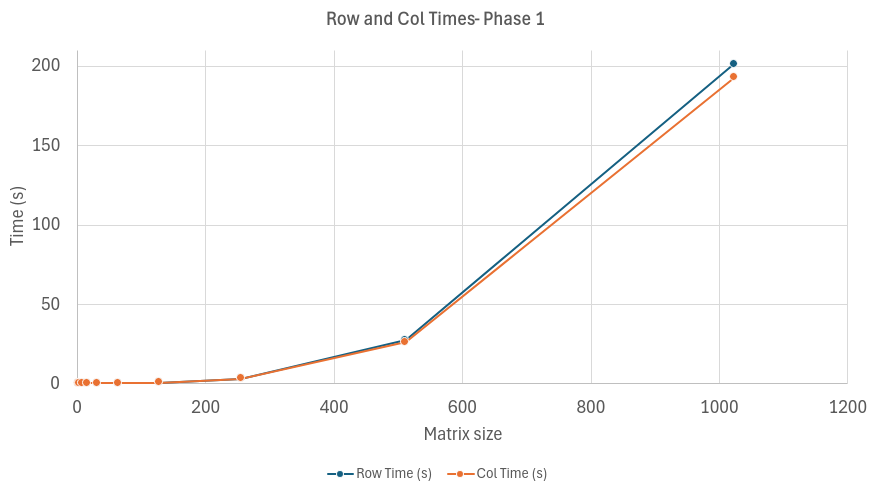
\includegraphics[width=0.65\textwidth]{img/1.png}
    \caption{Tiempos de ejecución de \rowmajor\ y \colmajor\ en \python}
    \label{fig:1}
\end{figure}

Se observa un crecimiento exponencial, tal como se esperaba y como sucederá en las siguientes fases, pero con unos tiempos de ejecución 
muchísimo más altos. \colmajor\ es ligeramente más rápido que \rowmajor, pero la diferencia es mínima. 

\newpage

Respecto al algoritmo de \zorder, en la \autoref{fig:2} se muestran los resultados obtenidos para los tamaños de matriz $512 \times 512$ y $1024 \times 1024$, los 
cuales se consideran los más representativos.

\begin{figure}[h]
    \centering
    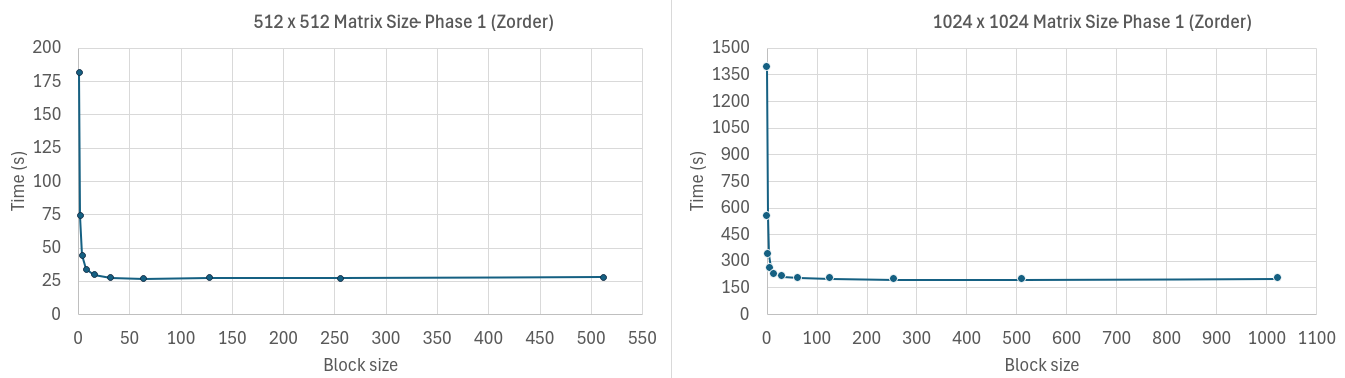
\includegraphics[width=0.95\textwidth]{img/2.png}
    \caption{Tiempos de ejecución de \zorder\ en \python\ ($N = 512$ y $N = 1024$)}
    \label{fig:2}
\end{figure}

Se observa una tendencia decreciente en ambos casos cuando el tamaño de bloque aumenta, si bien es cierto que resulta complicado determinar a simple vista un 
tamaño de bloque óptimo. De hecho, el uso de tamaños de bloque muy grandes (cercanos a $N/2$ e incluso $N$) produce un rendimiento muy similar al de 
tamaños de bloque pequeños ($4, 8, 16, 32 ...$), lo que sugiere que no se está aprovechando la idea del propio algoritmo. Teniendo en cuenta 
que en \python\ no se accede a memoria de la forma más eficiente, esta conclusión resulta bastante lógica.


Respecto a su comparación con \rowmajor\ y \colmajor, teniendo en cuenta los mejores resultados de \zorder\ para cada tamaño de matriz,
apenas mejora o iguala a los otros dos algoritmos. Quizá habiendo experimentado con tamaños de matriz aun mayores, se podrían haber 
obtenido resultados más favorables, pero en este caso no se ha considerado necesario debido a los tiempos de ejecución tan elevados. \\
En la \autoref{tab:2} se presenta la comparativa de los tiempos de ejecución de los los tres algoritmos, teniendo en cuenta el resultado más
óptimo de \zorder\ para cada tamaño de matriz.

\renewcommand{\arraystretch}{1.25}
\begin{table}[h]
    \centering
    \begin{tabular}{|c|c|c|c|}
        \hline
        Matrix size & \rowmajor\ (s) & \colmajor\ (s) & Best \zorder\ (s) \\ \hline
        $[...]$ & $[...]$ & $[...]$ & $[...]$ \\ 
        $64 \times 64$ & $0.046619$ & $0.046878$ & $0.047778$ \\
        $128 \times 128$ & $0.363829$ & $0.369213$ & $0.362896$ \\
        $256 \times 256$ & $2.933288$ & $2.948093$ & $3.007014$ \\
        $512 \times 512$ & $27.198958$ & $25.990449$ & $26.586173$ \\
        $1024 \times 1024$ & $200.909463$ & $192.439038$ & $193.267807$ \\ \hline
    \end{tabular}
    \caption{Tiempos de ejecución de los tres algoritmos en \python}
    \label{tab:2}
\end{table}